\documentclass[runningheads]{llncs}
\usepackage{graphicx}
\begin{document}
\begin{titlepage}
\centering
{\scshape\LARGE University of Potsdam \par}
\vspace{1cm}
{\scshape\Large Project in Computational Intelligence\par}
\vspace{1.5cm}
{\huge\bfseries Merging Robot Plans in the asprilo framework\par}
\vspace{2cm}
{\Large\itshape Adrian Salewsky\par}
\vfill
supervised by\par
Etienne Tignon
\vfill
{24.03.2021 \par}


\begin{abstract}
The asprilo framework was created to make plans for robots in a warehouse. It uses the language Answer Set Programming
which is a good choice for such a problem because this language was made for solving NP-hard problems. The solution works 
well for a small number of robots but at some point the computation time gets too high. This is why the idea came up to create plans
for a small number of robots and then combine the plans to get a working solution. This paper shows my approach on how to solve
the plan merging problem.
\end{abstract}
\end{titlepage}


\section{Introduction}
The asprilo framework is used to make plans for robots in a warehouse, i.e. when does a robot pick up or shelf or when does a robot move which way. 
It uses the language Answer Set Programming (ASP). Since there is no order in which ASP computes things, the predicates which describe the actions of robots and
the positions of objects contain an argument $T$ which declares at which time step the predicate holds. This project was done in the M-domain of the asprilo framework.
In the M-domain, the goal is to have a robot under each shelf that contains an ordered product at the last time step (the last time step is called horizon). This domain simplifies the framework 
to Multi-Agent Path Finding (MAPF). The framework works well for a small number of robots but for a high number of robots, the computation time gets too high. This is
why the plan came up to combine plans for a small number of robots to a plan for all the robots. During the combining of these plans, all the conflicts that arise between 
robots must be solved. This paper shows my approach on how to solve this plan merging problem in ASP. In the following section, I will show my general idea on how to solve 
conflicts. In the section after that, I will show my ASP encoding and explain its functions. Section 4 contains the analysis on the efficiency of my solution. The comparison of my approach with that of other groups that have
been working on the same project is shown in section 5. I will end my paper with a conclusion. 


\section{Idea}
The main idea behind my solution is that every time a conflict arises, one of the robots participating in the conflict randomly changes its movement during that time step and pushes his original plan back. 
To do that, the program needs to detect the conflicts and choose a robot who has to solve the conflict by generating a new move. The problem that arises is that
there is no option to overwrite predicates in ASP. Therefore, a new argument was needed for every predicate describing a plan. This new argument is called $conflict\_nr$ and 
the higher this argument is in a predicate the newer is the plan containing that predicate. This idea is a very simple approach to solving the problem since it completely adapts the original plan and only
inserts additional moves. This way the resulting solution might not have an optimal move set for every robot but it should be able to theoretically solve any problem instance.

\section{Answer Set Programming Encoding}
\subsection{Pre-Required Predicates}
To solve the problem there are several predicates needed before starting to solve the conflicts. There are two domain intervals whose upper bounds are constants: $time$ with the constant $horizon$ and $conflict\_nr$ with the constant $c\_nr$.
The constants are chosen at run-time. \\ There are some predicates that have been taken over from the encoding for the asprilo framework: $isRobot(robot(R))$ to check if something is a robot, $position((X,Y))$ to check if the node (X,Y) exists, $direction((X,Y))$ declares the 4 directions a robot can go into and $nextto(C1,D,C2)$ states that you get from the node C1 to the node C2 if you move into direction D. \\  
As input, the program expects a plan of the form $occurs(object(robot,R),action(move,D),T)$. This is transformed into the predicate $move(R,D,T,0)$. This means that the original plan has the $conflict\_nr$ 0. \\
Another part that has been mostly taken over from the encoding for the framework itself is the declaration of the position predicates:
\begin{verbatim}
position(R,C,0,0) :- init(object(robot,R), value(at,C)).
position(R,C,T,A) :- move(R,D,T,A), position(R,C',T-1,A), nextto(C',D,C).
                  :- move(R,D,T,A), position(R,C ,T-1,A), not nextto(C ,D,_).
position(R,C,T,A) :- position(R,C,T-1,A), not move(R,_,T,A), conflict_nr(A), 
                     isRobot(robot(R)), time(T).
\end{verbatim}
The difference is that position also contains an argument A for the $conflict\_nr$. The position only gets changed if a move in the same conflict depth A exists. The inertia rule also got changed accordingly. \\
The last part needed before the conflict solving is the predicate $goal$:
\begin{verbatim}
goal(R,C) :- position(R,C,horizon,0).
:- position(R,C,horizon,_), goal(R,C'), C!=C'.
\end{verbatim}
These rules declare that the last position of the initial plan is the goal position and that there can be no plan where a robot
is not on its goal position at the end. While this does not change the solution itself (the plan always only gets pushed back so the robot always ends on the same node), it improves the solution time. \\


\subsection{Conflict Detection and Selection}
There are two types of conflicts that can appear in a problem instance. The first one is that a robot arrives on a node which is either already occupied by another robot or another robot arrives in the same time step (see figures \ref{fig:c1_1} and \ref{fig:c1_2}).

\begin{figure}
   \begin{minipage}[b]{.4\linewidth} 
      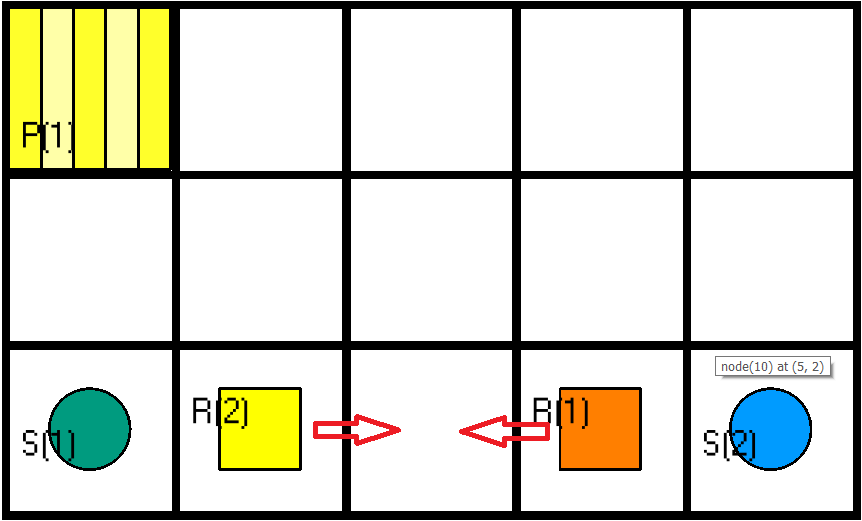
\includegraphics[width=\linewidth]{Images/Conflict 1_1}
      \caption{Two robots arrive on the same node at the same time step.}
      \label{fig:c1_1}
   \end{minipage}
   \hspace{.1\linewidth}
   \begin{minipage}[b]{.4\linewidth} 
      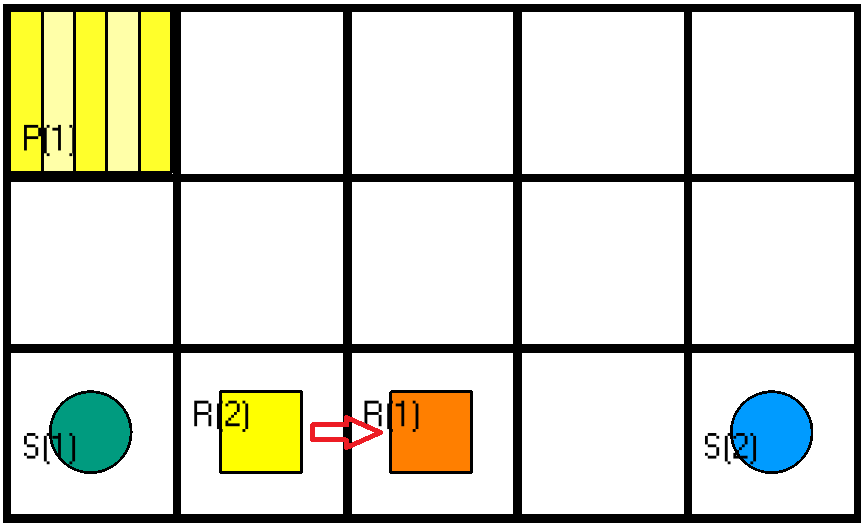
\includegraphics[width=\linewidth]{Images/Conflict 1_2}
      \caption{A robot moves to an already occupied node.}
      \label{fig:c1_2}
   \end{minipage}
\end{figure} 

\begin{verbatim}
conflict(R1,T,A) :- position(R1,C1,T-1,A), position(R1,C2,T,A), 
                    position(R2,C2,T,A), R1!=R2, conflict_nr(A).
\end{verbatim}
The predicate $conflict(R,T,A)$ is derived for the two robots participating in the conflict. \\
The second conflict is two robots switching their places (see figure \ref{fig:c2}):

\begin{figure}[h]
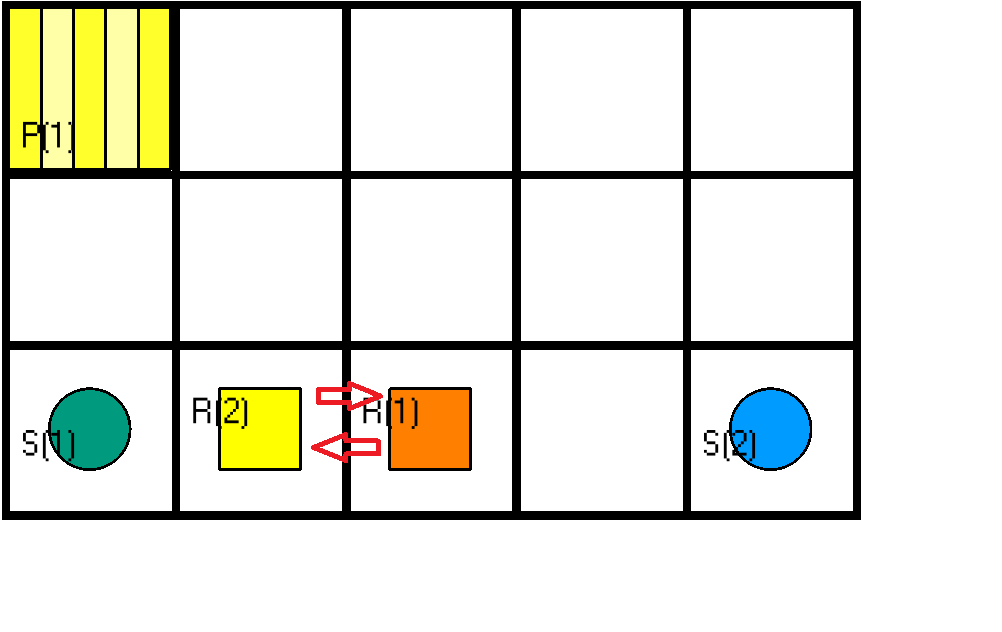
\includegraphics[width=75mm]{Images/Conflict 2}
\caption{Two robots switch places.}
\label{fig:c2}
\end{figure}

\begin{verbatim}
conflict(R1,T,A) :- position(R1,C1,T-1,A), position(R1,C2,T,A), 
                    position(R2,C2,T-1,A), position(R2,C1,T,A), 
                    R1!=R2, conflict_nr(A).
\end{verbatim}
The same predicate is derived for this type of conflict. \\
The program detects all of the conflicts arising in a plan this way. Only one conflict can get solved in each conflict depth, otherwise separate plans get created for each robot because there would be a separate plan to solve each conflict. The program chooses one of the conflicts that appeared the earliest.
\begin{verbatim}
1{solving_conflict(R,T,A) : conflict(R,T,A)}1 :- conflict(_,_,A).
:- conflict(_,T,A), solving_conflict(_,T',A), T'>T.
\end{verbatim}
The first rule declares that one conflict is chosen as the $solving\_conflict$ in each conflict depth. The second rule declares that a conflict cannot be chosen as solving conflict if there is a conflict that appears in an earlier time step in the same conflict depth. \\
This conflict selection makes it completely random which robot gets chosen as the one who has to solve the conflict. This could mean that the solver finds a plan where a lot of conflicts arise because of inefficient robot selection. This is why I have chosen to let the solver minimize the number of the conflicts:
\begin{verbatim}
#minimize {1,(R,T,A): solving_conflict(R,T,A)}.
\end{verbatim}
This rules forces the solver to find the most efficient way of selecting robots for the conflict solving.

\subsection{Conflict Solving}
After a robot is chosen as the conflict solver, its plan gets changed. 
\begin{verbatim}
0{move(R,D,T,A+1) : direction(D), nextto(C,D,_)}1 :- 
                  solving_conflict(R,T,A), position(R,C,T-1,A).
\end{verbatim}
The solver either chooses that the robot has to wait for this time step or that it moves into a random direction.
In both cases the $conflict\_nr$ has to rise for all robots:
\begin{verbatim}
position(R,C,T-1,A+1) :- solving_conflict(R',T,A), isRobot(robot(R)),
                         position(R,C,T-1,A).
move(R,D,T',A+1) :- solving_conflict(R',T,A), isRobot(robot(R)), R!=R', 
                    move(R,D,T',A), T'>=T.
\end{verbatim}
The first rule raises the conflict depth of the position predicate of every robot in the time step before the conflict. The second rule raises the conflict depth of every move predicate of every robot, except the selected one, in every time step after the conflict. This way only the predicates from the time step of the conflict and after that get changed. This reduces the amount of predicates compared to always changing all the predicates including the ones before the conflict happened. \\
The only thing left is to change the plan of the selected robot accordingly. Since there are two possible solutions for a conflict, there are two ways to push back the plan. The first possible solution is that the robot waits. In this case the plan only needs to get pushed back by one time step:
\begin{verbatim}
move(R,D,T'+1,A+1) :- solving_conflict(R,T,A), not move(R,_,T,A+1), 
                      move(R,D,T',A), T'>=T, time(T').
\end{verbatim}
The second possibility is that the robot moves into a random direction. If this is the case, the robot has to move into the opposite direction to be able to reach its goal position. The problem is that it is hard to decide at which time step the robot goes back since there could be new problems if it moves back at a time where there is already an occupied node which creates new conflicts. This is why, I let the solver decide at which time step the robot moves back:
\begin{verbatim}
1{step_back(R,(DX',DY'),T_B,A+1) : time(T_B), T_B<=horizon, T_B>T}1:- 
        solving_conflict(R,T,A), move(R,(DX,DY),T,A+1), DX'=-DX, DY'=-DY.
\end{verbatim}
This rule chooses a time step between the conflict and the horizon where the robot moves into the opposite direction of the dodge move. After that, the plan of the robot gets raised in conflict depth while changing the time steps accordingly:
\begin{verbatim}
move(R,D,T,A) :- step_back(R,D,T,A).
move(R,D,T'+1,A+1) :- solving_conflict(R,T,A), step_back(R,_,T_B,A+1), 
                      move(R,D,T',A), T'>=T, T<T_B-1.
move(R,D,T'+2,A+1) :- step_back(R,_,T_B,A+1), move(R,D,T',A), T'>=T_B-1.
\end{verbatim}
Since there are two rules in which the solver randomly decides which action to take, it is of advantage again to let the solver minimize the arising conflicts. This way the chosen actions result in the smallest number of conflicts.

\subsection{Integrity Constraints}
There are several integrity constraints used to ensure the correctness of the program as well as reducing the solution time.
These constraints only check if the predicates move out of the domain:
\begin{verbatim}
:- move(_,_,T,_), T>horizon.
:- position(_,_,T,_), T>horizon.
:- move(_,_,_,A), A>c_nr.
:- position (_,_,_,A), A>c_nr.
:- conflict(_,T,_), T>=horizon.
:- conflict(_,_,A), A>=c_nr.
\end{verbatim}
The conflict predicate cannot have $horizon$ or $c\_nr$ itself as argument because if a conflict arises the plan needs to get changed again and the predicates would move out of bounds.


\subsection{Output}
The resulting plan should only take the predicate with the highest conflict depth in each time step. 
\begin{verbatim}
new_move(R,D,T) :- move(R,D,T,MAX_C), MAX_C == #max{A: position(R,C,T-1,A)}.
\end{verbatim}
The predicate $new\_move$ contains the moves that had the highest conflict depth. The highest conflict depth is determined by looking at the position before a move. Every time a conflict arises, the position before the conflict has its conflict depth raised. This means that the position predicate is always the latest. The move predicate cannot be used to determine the highest conflict depth because there is no move predicate if a robot is waiting. \\
The predicate $new\_move$ gets translated into a form resembling the original input:
\begin{verbatim}
new_occurs(object(robot,R),action(move,D),T) :- new_move(R,D,T).
\end{verbatim}
The solver shows the $new\_occurs$ predicates as its solution.

\subsection{Extra Features}
There are two extra features I have dealt with. The first extra feature is the possibility of declaring that certain robots do not have to change their plan at all.
This is done by adding the predicate $strict\_plan(R\_ID)$ with $R\_ID$ being the ID of a robot. The only thing that gets changed in the encoding is in the conflict detection part:
\begin{verbatim}
conflict(R1,T,A) :- position(R1,C1,T-1,A), position(R1,C2,T,A), position(R2,C2,T,A), 
                    R1!=R2, conflict_nr(A), not strict_plan(R1).
\end{verbatim}
The only things that gets added is that a robot can only have a conflict that it might have to solve if it does not have the predicate $strict\_plan$. It is
the same for the second type of conflict. If two robots have a conflict and they both have strict plans there is no solution for that particular problem. 
This is encoded by using additional integrity constraints:
\begin{verbatim}
:- position(R1,C1,T-1,A), position(R1,C2,T,A), position(R2,C2,T,A), R1!=R2, 
   conflict_nr(A), strict_plan(R1), strict_plan(R2).
\end{verbatim}
The other conflict type looks the same. As this is a very hard constraint and can very easily lead to unsatisfiable problems, I have decided to extend the idea
to let the user control which robot gets chosen as the one who has to solve the conflict. This brings me to my second feature: Introducing a priority system.
The user can add predicates $priority(R\_ID, P)$ where $R\_ID$ is the ID of a robot again and P is the assigned priority of that robot. 
The solver then always chooses the robot with the lower priority to solve a conflict. If two robots have the same priority, either can be chosen. 
\begin{verbatim}
conflict(R1,T,A) :- position(R1,C1,T-1,A), position(R1,C2,T,A), position(R2,C2,T,A), 
                    R1!=R2, conflict_nr(A), p_priority(R1,P1), 
                    p_priority(R2,P2), P1<=P2.
p_priority(R,P) :- priority(R,P).
p_priority(R,0) :- not priority(R,_), isRobot(robot(R)).						
\end{verbatim}
The second conflict looks like the first one. The reason I change $priority$ to $p\_priority$ is that this way I can introduce a default value. If the user does not choose any priority value for a robot,
the priority gets set to 0. \\
Both features change how the conflict solving robot is chosen. Using them can be useful in certain scenarios, especially the second one, but it should be noted that those features can
easily make an instance unsatisfiable.

\section{Analysis of Solution}
There are several benchmarks the solution has been tested on a (a complete list can be found in the appendix). By looking at the results it is obvious that the presented solution is very time inefficient. While it is fast when there is only a small number of robots, a small $horizon$ and a small $c\_nr$, the solution gets very high very fast when these parameters are rising. It does not seem like there is a specific parameter that affects the time the most but that the time rises a lot as soon as there are at least 2 parameters rising. This time inefficiency was not entirely unexpected. There are several problems that result in this time inefficiency. The first one is that there are two domains whose upper bound are determined by a constant that is chosen at run-time. Especially the usage of the conflict depth makes it very inefficient. Every time there is a conflict, the whole remaining plan has to get pushed back. This results in a lot of predicates that need to be created. Another problematic part is the inertia rule. Since it has to check for every possible time step, conflict depth and robot whether there is a move predicate, it gets very inefficient. However, I have found no way to avoid this problem. \\
Another part that makes the solution inefficient is the usage of choice rules. Since there are several rules where the solver can decide which to choose, a lot of possibilities get created. However, this way of solving has the advantage that theoretically all problems can be solved. In practice, there is only one instance that was not solvable\footnote{Benchmark: Limited Moves by Marius and Niklas}. I have also created a similar benchmark\footnote{Benchmark: Instance 6} which basically deals with the same problem. The solver could solve this benchmark which means that there is another problem with the unsolvable instance that I could not find. Since it is likely a very niche problem instance, it is not too devastating that it is unsolvable. \\
To summarize, the solution is time inefficient but generally usable. To avoid a high solution time, the instances should be broken down to ones that only need smaller parameters. For example, big instances could be divided into smaller groups which get solved. After that these plans get combined again to form the complete plan. Another possible application case is already having a plan for a lot of robots and just adding a small number of robots. In both cases, the conflict number might be lower which would allow the solver to find a solution in an acceptable time frame.

\section{Comparison with other Approaches}
 - advantages and disadvantages of my approach compared to other approaches based on the benchmarking

\section{Conclusion}
This paper explained my approach on how to solve the plan merging problem for the asprilo framework. The solution is able to solve almost all of the benchmarks with the exception being a very niche 
benchmark that is unlikely to appear in the real world. There are two main problems in my solution. The first is that it is very time inefficient. The second is that the user has to input the time horizon and
the maximum conflict number. If he does not know it, he will likely take an upper bound which increases the computation time. While those two problems are definitely a major deficit of my solution, the trade-off
is that it is generally usable and it finds a solution with the minimum amount of conflicts needed to solve a problem instance. To avoid the time inefficiency, the user can also take a parallel approach, i.e. combining 
the plans of 2 robots at a time, then combining these plans again and so on. This way, the conflict number of the problem instances is likely lower than when combining all plans at once. This also means that the computation time
is reduced. Another possible usage of this solution is adding new robots to a warehouse where a plan for the other robots already exists. Since only a small number of robots is likely added, the conflict number is probably low
enough to get a solution in an acceptable time. \\
My solution to solving the plan merging problem has a lot of possibilities of getting improved, like time efficiency and taking it to the A-domain of the framework. Nevertheless, it is an approach that solves the problem and could
be used in certain scenarios.

\newpage

\begin{thebibliography} {6}
\bibitem{asprilo}
asprilo framework
\begin{verbatim}
https://asprilo.github.io/
\end{verbatim}

\bibitem{owngithub}
My Github Repository
\begin{verbatim}
https://github.com/salewsky/Plan-Merging
\end{verbatim}

\bibitem{github1}
Github Repository of Tarek Ramadan
\begin{verbatim}
https://github.com/tramadan-up/asprilo-project
\end{verbatim}

\bibitem{github2}
Github Repository of Tom Schmidt, Hannes Weichelt and Julian Bruns
\begin{verbatim}
https://github.com/tzschmidt/PlanMerger
\end{verbatim}

\bibitem{github3}
Github Repository of Marcus Funke and Maximilian Wiedenhöft
\begin{verbatim}
https://github.com/Zard0c/ProjektMAPF
\end{verbatim}

\bibitem{github4}
Github Repository of Marius Wawerek and Niklas Kämmer
\begin{verbatim}
https://github.com/NikKaem/mapf-project
\end{verbatim}

\end{thebibliography}

\newpage
\appendix
\section{Benchmark Results}
\begin{tabular}[h]{c|c|c|c|c|c}
Instance & Time & CPU-Time & Horizon & Solved Conflicts & Robots \\
Instance 1 & 0.125s & 0.109s & 5 & 1 & 2 \\
Instance 2 & 5.063s & 5.016s & 10 & 3 & 4 \\
Instance 3 & 2.672s & 2.641s & 9 & 2 & 4 \\
Instance 4 & 0.078s & 0.078s & 2 & 0 & 4 \\
Instance 5 & 0.484s & 0.469s & 4 & 3 & 4 \\
Instance 6 & 696.239s & 695.594s & 14 & 9 & 2 \\
Instance 7 & 134.847s & 134.672 & 9 & 3 & 8 \\
\end{tabular}

\end{document}